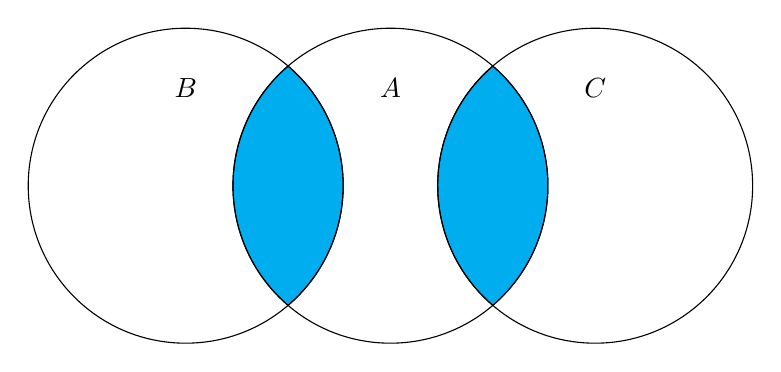
\begin{tikzpicture}
    % Coordinates for the points.
    \coordinate (B) at (-2.6, 0.0);
    \coordinate (A) at ( 0.0, 0.0);
    \coordinate (C) at ( 2.6, 0.0);

    % Fill in the overlap between B and A.
    \draw[fill=cyan] (-1.3, -1.51987) arc(-49.46:49.46:2) arc(130.54:229.46:2);

    % Fill in the overlap between A and C.
    \draw[fill=cyan] (1.3, -1.51987) arc(-49.46:49.46:2) arc(130.54:229.46:2);

    % Draw circles outlining the regions A, B, and C.
    \draw[draw=black] (A) circle (2);
    \draw[draw=black] (B) circle (2);
    \draw[draw=black] (C) circle (2);

    % Add some labels.
    \node at (A) [above=1cm] {$A$};
    \node at (B) [above=1cm] {$B$};
    \node at (C) [above=1cm] {$C$};
\end{tikzpicture}